
%\documentclass{sig-alternate-05-2015}
\documentclass[conference]{IEEEtran}



\usepackage{microtype}
%\usepackage{mathptmx}
%\usepackage[scaled=.90]{helvet}
%\usepackage{times}

%\usepackage{mathtools}
\usepackage{multirow}
\usepackage{graphicx}
\usepackage{algorithm}
\usepackage{algorithmic}
\usepackage{color}
\usepackage{caption}
\usepackage{paralist}
\DeclareCaptionType{copyrightbox}
%\usepackage{subcaption}
\newtheorem{definition}{Definition}
\usepackage{amsmath}
\usepackage{url}
\usepackage{algorithm}
\usepackage{algorithmic}
\usepackage{booktabs}
\usepackage{amssymb}
\usepackage{url}


%\usepackage{subfigure}
\usepackage[skip=1pt]{subcaption}

\usepackage{graphics}


\graphicspath{ {figures/} }

\newcommand{\myparatight}[1]{\smallskip\noindent{\bf {#1}:}~}

\renewcommand{\algorithmicrequire}{\textbf{Input:}}
\renewcommand{\algorithmicensure}{\textbf{Output:}}
\newcommand{\todo}[1]{{\textcolor{red}{{\bf TODO:} #1}}}
\newcommand{\tabincell}[2]{\begin{tabular}{@{}#1@{}}#2\end{tabular}}

\newcommand{\DB}{\ensuremath{\mathcal{ST}}}
\newcommand{\RR}{\ensuremath{\mathbb{R}}}
\newcommand{\NN}{\ensuremath{\mathbb{N}}}
\newcommand{\clust}{\ensuremath{\#\mbox{Clust}}}

\newcommand{\TODO}[1]{{\bf \textcolor[rgb]{1.00,0.00,0.00}{TODO: #1}}}

\newcommand{\argmin}{\operatornamewithlimits{argmin}}
\newtheorem{example}{Example}




\begin{document}



\title{A Recurrent Neural Network Framework for Spatio-Temporal Site Recommendation}

%\author{Blinded for Double-Blind review\vspace{2cm}}
\author{\IEEEauthorblockN{Guolei Yang}
\IEEEauthorblockA{Iowa State University\\ Ames, IA, USA\\
yanggl@iastate.edu}
\and
\IEEEauthorblockN{Andreas Z\"ufle}
\IEEEauthorblockA{George Mason University\\ Fairfax, VA, USA\\
azufle@gmu.edu}
} 
%\author{\IEEEauthorblockN{Maximilian Franzke, Tobias Emrich} \IEEEauthorblockA{
%Ludwig-Maximilians-Universit\"at\\
%Munich, Germany\\
%\{franzke, emrich\}@dbs.ifi.lmu.de}
%\and
%\IEEEauthorblockN{Andreas Z\"ufle, Matthias Renz}
%\IEEEauthorblockA{George Mason University\\ Fairfax, VA, USA\\
%\{azufle, mrenz\}@gmu.edu}
%\and
%\IEEEauthorblockN{James Kirk\\ and Montgomery Scott}
%\IEEEauthorblockA{Starfleet Academy\\
%San Francisco, California 96678-2391\\
%Telephone: (800) 555--1212\\
%Fax: (888) 555--1212}
%}
%\author{\IEEEauthorblockN{Maximilian Franzke, Tobias Emrich\\} \IEEEauthorblockA{Institute for Informatics\\
%Ludwig-Maximilians-Universität\\
%Munich, Germany\\
%\{franzke, emrich\}@dbs.ifi.lmu.de}
%\and
%\IEEEauthorblockN{Andreas Züfle, Matthias Renz\\}
%\IEEEauthorblockA{George Mason University, Fairfax, VA, USA   \\
%\{azufle,mrenz\}@gmu.edu}
%}
\maketitle



\maketitle
\vspace{6cm}


\begin{abstract}

\end{abstract}


%
% The code below should be generated by the tool at
% http://dl.acm.org/ccs.cfm
% Please copy and paste the code instead of the example below.
%
%\begin{CCSXML}
%<ccs2012>
% <concept>
%  <concept_id>10010520.10010553.10010562</concept_id>
%  <concept_desc>Computer systems organization~Embedded systems</concept_desc>
%  <concept_significance>500</concept_significance>
% </concept>
% <concept>
%  <concept_id>10010520.10010575.10010755</concept_id>
%  <concept_desc>Computer systems organization~Redundancy</concept_desc>
%  <concept_significance>300</concept_significance>
% </concept>
% <concept>
%  <concept_id>10010520.10010553.10010554</concept_id>
%  <concept_desc>Computer systems organization~Robotics</concept_desc>
%  <concept_significance>100</concept_significance>
% </concept>
% <concept>
%  <concept_id>10003033.10003083.10003095</concept_id>
%  <concept_desc>Networks~Network reliability</concept_desc>
%  <concept_significance>100</concept_significance>
% </concept>
%</ccs2012>
%\end{CCSXML}
%
%\ccsdesc[500]{Computer systems organization~Embedded systems}
%\ccsdesc[300]{Computer systems organization~Redundancy}
%\ccsdesc{Computer systems organization~Robotics}
%\ccsdesc[100]{Networks~Network reliability}


%
% End generated code
%

%
%  Use this command to print the description
%
%\printccsdesc

% We no longer use \terms command
%\terms{Theory}

%\keywords{graph mining, social networks, attributed graph, non-redundant, overlapping, parameter-free}

\section{Introduction}\label{sec:intro}

The prevalence of GPS-enabled device such as  smart phone leads to the thrift of many Location-Based Services (LBS) including GoogleMap and Foursquare, where users can access the information of millions of Point-of-Interests (PoIs) like restaurants and shopping centrers. More and more customers relies on such LBS to search for PoIs of their interest on a daily basis. An important type of PoI information users are looking for on such LBS is \textbf{PoI rating}, i.e., a ``score" that measures how good the PoI is in terms of service provided. For example, on GoogleMap, each PoI is rated on a scale of 1 to 5 ``stars". The more stars a PoI has, the higher it is rated, reflecting that the PoI offers services of high quality.

PoI rating plays a crucial role in customers' decision making process. Obviously, a user is more likely to use the service of PoIs with higher ratings, comparing with similar (in terms of location and price), but lower-rated PoIs. PoI rating is also an important factor that affects the rank of a PoI in the search result return to a user. Additonally, it is used to determine whether a PoI is to be recommended to users by many recommendation systems. For the above reasons, PoI rating is crucial to the owner a the PoI, and this rating also provides important insights on how to improve his business in order to attract more customers.

A fundamental requirement for PoI rating is it should accurately reflect the quality of service of the PoI. On LBS, PoI rating is usually automatically generated via a data mining process, which takes into consideration of several factors. Such factors usually include individual user's explicit rating and review of the PoI, location and category of the PoI, etc. (e.g., ). This rating generation method is similar to the product rating system for online shopping websites such as eBay and Amazon, which is known to be suffering from several problems, such as:

1. A major concern of this system is it is vulnerable to \textbf{shilling} attacks. Shilling attack refers to the behaviour of giving fake ratings and reviews to products, in order to manipulate their ratings. Its effectiveness has been shown by several studies on user-rating based product rating systems. Due to the aforementioned reasons, PoI owners strive to improve their ratings and some of them may resort to this attack. It is estimated that -\% of user rating on ... are likely to be fake. Since anyone can rate PoIs on LBS such as GoogleMaps, there is no reason to believe that their PoI rating systems are immune from such attacks. 

2. This system relies on complex text-mining algorithms. Written review is usually more trustworthy and provides more information about a product comparing with simple a rating score. However, extract useful rating information (e.g., positive/negative labels) from written reviews is known to be a challenging task. Although a few methods has been proposed for automatic review-text mining, the mining process is still expensive and the accuracy is not very satisfactory. More importantly, when used for PoI rating generating, the errors from multiple user's review will accumulate. 

3. The system requires extra user efforts and may not be objective. It require users to explicitly give their ratings to a location and/or write reviews, which requires extra user efforts and may not be objective (e.g., a ``score" can be interpreted very differently by different users, inaccurate description, only users who strongly dislike or like the PoI are motivated to rate or write reviews, etc.). 

The root of the above problem is that this method strongly relies on individual user's explicit ratings and written reviews, but their actual behaviours. However, a unique difference between a PoI and a normal product is that for a PoI, an LBS can not only know who visited it, but also knows the trajectories of these visitors. This is made possible by either keep tracking user's locations, or ask users to voluntarily report check-in to the PoI. For example, the publicly available Foursquare dataset contains more than 3 millions of user self-reported check-ins.

These trajectories provides a unique dimension that could be leverage for PoI rating, which provides a possible solution to the aforementioned problems of normal product rating method. To this end, we study the spatio-temporal PoI rating prediction problem. We aim to answer the following question: \textit{Is it possible to accurately predict the rating of a PoI by mining the trajectories of its historical visitors?} We want to point out that our problem is different from user-location rating prediction, where the goal is to predict whether \textit{a specific user} likes a PoI, but not to predict the overall rating of a PoI. The former finds its applications in making personalized recommendations, while the later is crucial for the aforementioned applications.

There are several potential advantages of using trajectory data for PoI rating: (i) It is prone to alteration by fake-user-ratings and spam/bot-user-ratings. It is much harder and more expensive to forge a valid trajectory than to submit a fake rating score or review. As such, it is resistant to common shilling attack. {ii} It does not require an intermediate process to extract label information from written reviews. (iii) no extra user effort to capture their opinions such as filling in rating forms or submit a written review, and (iv) it is based on user's behaviour, thus could be more objective.

A straightforward way to predict the rating of a PoI is to simply count the number of visitors. This is based on the assumption that high-rating PoIs are usually popular locations since they are more attractive to costumers. Although the assumption is reasonable to some extend, it has some obvious drawbacks. First, a PoI being popular could only be the result of its location. For example, a Starbucks coffee shop located in a busy airport could have much more visitors than another Starbucks in suburb area, despite that the products they serve is largely the same. Second, user's choice of PoIs may be affected by time. For example, a customer who is on the way to work is likely to choose a restaurant for breakfast only because it is close to work and serves food fast, not because the food is exceptional. Third, the visits from different user may different predictive power since some user may be more selective in choosing PoIs in certain circumstance. For example, a user who is more familiar with an area may knows better which restaurant have the best service.  


To address the above challenges, we propose a \textit{visiting-pattern-based PoI rating prediction framework} that captures the spatio-temporal characteristic of visits. The visiting-pattern is extracted from a user's trajectory, which reflects how often the user visits a PoI, the visiting time, and the travel distance. The proposed framework is based on a comprehensive analysis of the intuitive relation between user visits to a PoI and its rating over the Foursquare dataset. The core the proposed framework is a novel regression model that takes into consideration the difference between visitors, visiting time, PoI locations, etc. We show in experiments on real world dataset that the proposed method outperforms not only the simple counting based method, but also the method based on state-of-the-art user-location rating techniques. We summarize our contributions as follows:
\begin{itemize}
\item We formally define the spatio-temporal PoI rating problem, and conduct the first systematic study of the problem.

\item We perform a comprehensive analysis of the Foursquare check-in dataset, in order to identify relations between user visits and PoI ratings.

\item Based on our analysis, we propose a visiting-pattern-based PoI rating prediction framework. It captures the spatio-temporal characteristic of visits by extracting patterns from user's trajectories. The core the proposed framework is a novel regression model that takes into consideration the difference between visitors, visiting time, PoI locations, etc. 

\item The proposed technique is implemented and evaluated on real world dataset. The results show it outperforms not only the simple counting based method, but also the method based on state-of-the-art user-location rating techniques.
\end{itemize}


The rest of this work is organized as follows. We survey the state-of-the-art on location rating in Section \ref{}. Then, we formally define the problem spatio-temporal PoI rating in Section \ref{}. Section present our analysis of the Foursquare check-in dataset. Details of the proposed framework is described in Section \ref{}. Our solution is evaluated in Section \ref{}. And finally, we conclude our work in Section \ref{}.  

\section{Related Work}\label{sec:rw}

In a recommender system, there is a set of users and a set of items. The goal of the system is to recommend a user certain items that best match the user's preference. The essential research problem here is, how to predict a user's rating for items that were not rated by him. This is due to the fact that the number of users and items are usually very large, and it is impractical to ask users to rate every item. We study this problem in the context of user-site recommendations.

Two types of recommender systems have been developed in the past few decades. \textbf{Content-based recommender systems} (e.g., \cite{contentbasedLang95,contentbasedPazzani97}) analyze properties of item (e.g., item descriptions) and/or user profile to identify items that are attractive to the user. The spatial-temporal features or visiting patterns we explored is similar to this type of recommendation. Nevertheless, existing methods mostly focus on features extracted from user's interaction with the recommender system (e.g., view or purchase history, reviews, user profile).

The other type is \textbf{Collaborative-filtering recommender systems} (e.g., \cite{userUserRec94,amazonRecommendation,MFRec09})). Collaborative-filtering predicts users' preference to items based on their similarity to other users. It relies on analysis of large amount existing product rating data. However, it becomes challenging to calculate user-similarity when there is not enough such data. This is known as the cold-start problem. A widely used technique for collaborative-filtering is Matrix factorization~\cite{koren2009matrix}. Matrix factorization works on a user-item rating matrix. It models both users and items as vectors of latent features.

Our work is different from existing Location Recommendation in LBSN~\cite{yu2015survey, ye2010location,wang2013location, cheng2012fused}, which also considers PoIs as recommended items. They propose to explore geo-social activities of users to facilitate the identification of users with similar preference in matrix factorization. For example, users demonstrate similar location-visiting pattern is likely to have similar rating for PoIs, therefore co-visitation of locations can be used as a measurement for similarity between users. Most works in this category combines check in data with additional information (e.g., social connection and/or user profile). These techniques fall in the category of collaborative-filtering. In contrast, our work is to direct predict a user's preference purely based on explicit features extracted from his trajectory, which is a fundamentally different approach and was not investigated in literature to our knowledge.
\section{Problem Definition}
\label{sec:probdef}
In this section we formally define a user-trajectory, and define our notion of a user-site-stay, which we are going
to use to extract features to estimate the affinity between a user and a site later in Section \ref{sec:method}.
We first start by defining a trajectory as follows.
\begin{definition}[Spatio-Temporal Database]
Let $\mathcal{U}$ denote a set of unique user identifiers, let $\mathcal{G}=[-90,90]\times [-180,180]$ denote the space of longitude/latitude geo-coordinates, and the $\mathcal{T}$ denote the time domain.
A \emph{spatio-temporal database} $\DB\subseteq \mathcal{U}\times \mathcal{G}\times \mathcal{T}$ is a collection of triples $(id\in\mathcal{U},(lat,long)\in\mathcal{G},t\in\mathcal{T})$. Each triple $(u,s,t)\in\DB$ is called an observation.
\end{definition}
We group a spatio-temporal database into observations of the same user, denoted as user-trajectory, formally:
\begin{definition}[User-Trajectory]
Let $\DB$ be a spatio-temporal database and let $u\in\mathcal{U}$ be a user. The set
$$
\DB(u):=\{(u^\prime,(lat,long),t)\in\DB|u=u^\prime\}
$$
is called the user-trajectory of user $u$.
\end{definition}
In order to obtain recommendation information from a user-trajectory, we need to link the user-trajectory to sites, such as restaurants and hotels. For this purpose, we join a spatio-temporal database with a database of points of interest (such as provided by Open-Street Map) like restaurants and hotels. Next, we define our notion of a \emph{stay}. A stay is an event of user visiting a site, enriched by the duration of the stay.
\begin{definition}[Stay Trajectory]
Let $\DB$ be a spatio-temporal database and let $\mathcal{S}\subseteq \mathcal{G}$ be a collection of $(lat,long)$ pairs of sites. A stay is a triple $(u\in U,s\in\mathcal{S},(t_\text{start},t_\text{end})\in T\times T)$, indicating that user $u$ has stayed at site $s$ from time $t_{start}$ to time $t_{end}$.
We let $(\DB\bowtie\mathcal{S})$ denote the set of all stays mined from all trajectories $\DB$ using all sites in $\mathcal{S}$.
The sequence of all stays a user $u\in\mathcal{U}$ is called the stay-trajectory $(\DB\bowtie\mathcal{S})(u)$ of $u$, defined as:
$$
(\DB\bowtie\mathcal{S})(u):=\{(u,p,(t_\text{start},t_\text{end}))\in\mathcal{S}|u=u^\prime\}
$$
\end{definition}
Finding stay points in trajectory and PoI databases is a research topic that has raised attention in the past. In this work, we make the explicit assumption that stay points of a trajectory are already given, as we use trajectory datasets where stay points are explicitly labeled. We discuss this assumption and related work on stay-point detection in Section \ref{sec:stay}.

Given stay-trajectories for each user, the challenge of this work is to predict the rating between users and a site. As site is PoI which can be rated by a user, such as a restaurant or a hotel. We assume that we have a recommendation database, where users can rate sites. We assume normalized rating values in the interval $[0,1]$, where $0$ corresponds to the lowest rating and $1$ corresponds to the highest rating.
\begin{definition}[User-Site Recommendation Database]
A recommendation database $\mathcal{R}$ is a set of user ratings $\mathcal{R}\subseteq \mathcal{U}\times\mathcal{S}\times [0,1]$.
\end{definition}
The task of this work is to predict the triples in $R$. That is, the challenge is to predict the rating that a user $u\in \mathcal{U}$ will give to a site $s\in\mathcal{S}$, using a spatio-temporal given in $\DB$.


\section{Data Analysis}\label{sec:analysis}
The first step of our user-site-recommendation approach requires to map a raw trajectory $\DB(u)$ of a user $u$ to a stay-trajectory $(\DB\bowtie\mathcal{S})(u)$. Such stay points can be detected by using existing work such as proposed in \cite{li2008mining,zheng2009mining,zheng2010geolife,xiao2010finding}. All of these works use a distance threshold $\theta_{d}$ and defines a stay as the duration of time where the trajectory does not exceed a distance of $\theta_{d}$ to a PoI. In this work, we entirely circumvent the step of implicit stay point detection, by using data that has explicit stay points. Therefore, in our experimental evaluation we use Check-in data from location based social networks (LBSNs), which explicitly contain the stay points of users. Clearly, by circumventing the problem of stay point detection, we limit our experimental evaluation to LBSN Check-in data, which is relatively small (hundreds of megabytes of data), compared to large raw trajectory databases (Terrabytes of data).
Yet, we postulate that our relatively small FourSquare Check-in dataset, allows to effectively predict the user rating of a restaurant. This hypothesis is also supported by our experiments. 
%
%While we circumvent the problem of stay point detection by using Check-in data, we still need to estimate the duration of stay, as the duration of a stay is one of the features that we will use for prediction in Section \ref{?}. Thus, we interpret each Check-in $c$ as a stay point. If the corresponding user has no other check-ins for the next six hours, we set the duration of $c$ to \emph{UNKNOWN}. Otherwise, the set the duration to the time in-between these two check-ins. 
\section{Proposed Method}\label{sec:method}

Our goal is to extract a set of spatial-temporal features from a user's trajectory, which can be directly used to predict the rating of a PoI. There are many features that could potentially be related to a user's feeling of a PoI. We discuss in this section a set of common features we select for the rating prediction problem, and the methods we use to extra such features. It is easy to understand why these features are selected since they are intuitive.

\subsection{Extracting the frequency of visits of a user}

Our assumption is, if a user repeatedly visits a PoI, e.g., always dine in the same restaurant, it strongly suggests that the user favours the PoI. On the other hand, if a user visits a PoI only once and never comes back, it suggests the user dislike the place. Therefore we choose the frequency of visits as a feature. Here, each stay-point is considered a visit.

In order to extra frequency information from a user's trajectories, we count for how many time the user visits a PoI in a given time period. Each check-in to the PoI is counted as one visit. Users are then assigned into several frequency groups (Table~\ref{frequencyGroups}) based on how often they visit the PoI. Note that if a user has never visited a PoI, he cannot rate it. Thus we do not assign any group for such users.

\begin{table}[htbp]
\begin{center}
\caption{Groups based on how often user visits a location \label{frequencyGroups}}
\begin{tabular}{|l|l|} \hline
ID & \textbf{Frequency groups} \\ \hline
1 & At least one visit per day \\ \hline
2 & At least one visit per week \\ \hline
3 & At least one visit per month \\ \hline
4 & Less than one visit per month \\ \hline
\end{tabular}
\end{center}
\end{table}

We note a user's behaviour may vary over time. For example, if a user likes a shopping center, he may visit a shopping center very frequently during Thanksgiving and similar holidays, while visit the same place only once in several month during the rest of the year. As a result, the timing window used to count visits can have significant impact on the user's group assignment. For the same user, if we consider only visits happened in the Thanksgiving week, the user belongs to the ``At least one visit per week " group. However, if we look at the year-long visits, he may be grouped into ``Less than one visit per month" since his visits are averaged over twelve months. We propose a simple way to mitigate this problem.

First, we use timing windows with different sizes simultaneously to compute the frequency of visits of a user. Specifically, given a user's trajectory data for a period of $n$ days, for each week/2 weeks/month within these $n$ days, we count the number of visits that falls in the same week/2 weeks/month. We then use this count to compute the user's group of that specific period. Here we use week and month as nature timing windows, but in practice the size of timing window can be arbitrary. Second, when a user's visit frequency demonstrates inconsistency in different time period with the same timing window size, we use his maximal visiting frequency, e.g., if a user visits a location 3 times a week in week 1, but 0 times in week 2, the user is then categorized as ``At least one visit per week" in this case. 

Additionally, for each PoI, we calculate three numerical features that also describe a user's visiting pattern to the PoI: 1) \textbf{Average duration between two consecutive visits of the user}, 2) \textbf{Minimal duration between two consecutive visits of the user}, and 3) \textbf{Maximal duration between two consecutive visits of the user}. These information are supplemental to the frequency groups. 

%We are interested in finding out their impact on the rating prediction result.

\subsection{Extracting the length of stays of a user}

Given a trajectory of a user, the length of stays can be inferred by examining the interval between consecutive check-ins of the user. If two visits are reported within a time threshold $\tau$, e.g., 30-minutes, it is safe to consider the two check-ins belong to the same stay. Thus, the minimal length of this stay is the time frame between the two check-ins. Similarly, an upper bound of the length of stay is the time between a check-in to the location and the closest check-in to a different location. This provides us with a coarse way to estimate the average length of stay of users to a PoI. This method is most accurate if the user's location is reported periodically with small intervals, or whenever the user changes location.

\subsection{Extracting the travel distance of a user from its home base}

If a user is willing to travel a long distance from his home/work area to a PoI, it is likely that the PoI is attractive to him. Unfortunately, measuring the travel distance from one's home/work can be challenging. This is because users' home or work address or coordinates are usually not explicitly marked in a spatial-temporal dataset due to privacy concerns.

We use distance-based location clustering (e.g., weighted k-means~\cite{kerdprasop2005weighted}, where the weight of a location is the number of visits by the user) to estimate a user's home base, i.e., an area where he is likely to live/work. Locations a user visits frequently is likely to formulate a dense cluster in the area where he lives and works~\cite{golle2009anonymity, zang2011anonymization}. If there exists a location that is isolated from any of these clusters, we deem such a location as ``far from home". It requires extra effort for the user to travel this location. Willing to make such effort indicates the user may like the place. An example of home base and isolated locations is illustrated in Figure~\ref{example}.

\begin{figure}[htb]
\center
%\vspace{-2mm}
{\includegraphics[width=0.45 \textwidth]{homebase.pdf}}
%\vspace{-12mm}
\caption{Example of home base and isolated locations} 
\label{example}
%\vspace{-4mm}
\end{figure}

For each isolated location, we estimate the travelling effort for the user to reach the location. Using the distance between the isolated location and the user's home base may be biased. A user who likes to drive can easily travel to a mall several miles away from home, but for someone who does not have a car, travelling the same distance means significantly more effort. Instead, we use the relative travelling distance. For a location $l$, we compute $D_l = d_l / \overline{d_{home}}$ where $d_l$ is the minimal travel distance between $l$ and any home base location, and $\overline{d_{home}}$ the average travel distance between locations within the user's home base.

\subsection{Extracting the type of PoI}

A user's spatial-temporal behaviour can be very different in different types of PoIs. Suppose a user gives high rate for both a coffee stand and a theatre. It is common for a user to visit the coffee stand every day or even multiple times a day, while such a visiting pattern is not likely to appear for his visiting to the theatre. Given the diversity of locations, we believe the type of different PoIs serves as an important feature in the rating prediction process.

Fortunately, in many spatial-temporal datasets (e.g., \cite{yang2014modeling}), a category is given for each PoI. Nevertheless, a dataset may provide only coordinate of visited locations with no additional information. One way to infer the type of PoI in this case is to match the coordinates to PoIs using geo-info systems such as GoogleMap, which provides detailed category information of PoIs.

\subsection{Discussion}

Due to limited space, we briefly discuss some other useful features that we conjecture are related to users' rating of PoIs.

\myparatight{Regional difference} User's visiting pattern to some PoIs can be region-sensitive. Consider an example of two restaurants. Restaurant A locates near a busy train station while restaurant B is in suburb region. Even if the B provides better service than A, A may attract much more visitors comparing with B due to its better location. A possible way to mitigate the problem is to add a feature that describes region of a location (e.g., ``Downtown region", ``Less popular region", etc.) but it requires extra geo-demographic information which cloud be hard to collect. A simpler and efficient way is to explore the relation between nearby PoIs of the same type. The reason is intuitive. For example, given several restaurants close to each other, if all of them are visited by 100 users per day, except for one restaurants which has only 10 visitors per day, it is very likely that this restaurants has a bad rating.

\myparatight{Scale of the PoI} It is worth mentioning that the scale of a PoI has an obvious impact on the total number of visits to it. A small convenient store, regardless of how users like it, is not likely to have even close number of visitors comparing with a large super market. However, to our knowledge, these is no convincing way that can accurately estimate scale of a PoI. We leave this for future exploration when such data is available.

\myparatight{Social connection between users} The prevalence of LBSNs makes it easy to learn social connects between users. If several users who are socially connected check in at a PoI at the same time, it is likely that they have a group social event at the PoI. The fact that a group of friends choose to meet at a PoI suggests most of the users in the group like the place. We may also assume a user's rating of some PoIs is affected by the rating of his friends, given that they frequently visit a similar set of PoIs. In general Group-visits may demonstrate different pattern comparing with individual visits, and therefore can be used as a distinguished feature. 

%!TEX root = ./main.tex
\section{User-Site Rating Prediction}
\label{sec:prediction}

Given a set of user trajectories and a set of PoIs visited by these users, we aim at predicting the users' rating for each of the PoI. The rating is usually expressed as a numeric score. We assume the score is no-negative and can be continuous. A higher score corresponds to a better user rating. We propose to use out-of-the-box machine learning algorithms to training the prediction model with the aforementioned spatial-temporal features as input. In order to learn the model, we assume the accurate ratings from some users for certain PoIs are given. This information can usually be extracted from websites that provide reviews of PoIs, such as Yelp, FourSquare, GoogleMap, and TripAdvisor. 

We do not intend to explore existing machine learning techniques in an encyclopaedia way to find the most effective one for our problem. Instead, our goal is to demonstrate the spatial-temporal features of a user has the potential to predict his rating of PoIs he visited. To this end, we choose two representative techniques, \textbf{linear regression} and the standard \textbf{deep neural networks} (DNN)~\cite{schmidhuber2015deep}. Linear regression is chosen due to its simplicity; Deep neural network, although is much more expensive to train, demonstrates good performance in many applications (e.g., \cite{ruiz2013innovative, hinton2012deep, krizhevsky2012imagenet}).

A DNN is a artificial neural network with more than one hidden layer. Each hidden layer consists of certain number of hidden units or neurons. A hidden unit $i$ uses a output function $f(x_i) = y_i$ to map its input $x_i$, received from the previous layer, to an output $y_i$, which is then sent to the next layer. Typical output functions include linear, logistic, sigmoid, softmax, etc. In our experiments, we construct a DNN with a simple fully-connected 4-layer architecture. The DNN is discriminatingly trained by backpropagation. A cost function is used to measure the discrepancy between the target output and predicted value in backpropagating. For our problem, we use Mean Square Error (MSE) as cost function. 

Since we are dealing with a relatively small number of features, here we will not concern ourselves with the problem of handling overfitting and optimizing of training time.
%\section{Spatio-Temporal Trend Dissemination Rule Mining}\label{sec:mining}
This section describes our approach at mining spatio-temporal trend
dissemination rules. As a first step, we need to acquire past trends, to mind
dissemination rules from. For this purpose, we apply existing textual trend
mining solutions proposed in the recent past, which are briefly sketched in
Section \ref{subsec:Signi} for self-containment. Next, as a second step used for
preprocessing, we employ a space composition scheme in Section
\ref{subsec:decomp} to ensure having a similar number of tweets in each spatial
region using a k-d tree.
As a third step, we model the flow of trends over space and time in Section
\ref{subsec:tensor}. Therefore, we transform a \emph{trend count matrix}, as
defined in Definition \ref{def:trendcountmatrix}, into a \emph{trend flow
tensor}, which describes the flow from any source region to any target region at any
point in time for any trend. Consequently, constructing a \emph{trend flow
tensor} for each trend that we mined in the first step, yields a four-mode Space
$\times$ Space $\times$ Time $\times$ Trends tensor, which will be fed to our
fourth step, the mining step. In the mining step proposed in Section
\ref{subsec:mining}, we employ a tensor factorization approach to discover
latent features of trends, latent features of trend-source-regions and latent
features of trend-target-regions. These latent features allow us to cluster
trends into sets of trends which disseminate similarly over space and time.
Then, for each cluster of similar trends, we obtain trend flows from the
\emph{reconstructed trend flow tensor}.

\subsection{Traditional Trend Mining}
We use SigniTrend \cite{schubert2014signitrend}. {\bf Micheal: Insert a third of
a column of description of signitrend here for self-containment. PLACEHOLDER
PLACEHOLDER PLACEHOLDER PLACEHOLDER PLACEHOLDER PLACEHOLDER PLACEHOLDER
PLACEHOLDER PLACEHOLDER PLACEHOLDER PLACEHOLDER PLACEHOLDER PLACEHOLDER
PLACEHOLDER PLACEHOLDER PLACEHOLDER PLACEHOLDER PLACEHOLDER PLACEHOLDER
PLACEHOLDER PLACEHOLDER PLACEHOLDER PLACEHOLDER PLACEHOLDER PLACEHOLDER
PLACEHOLDER PLACEHOLDER PLACEHOLDER PLACEHOLDER PLACEHOLDER PLACEHOLDER
PLACEHOLDER PLACEHOLDER PLACEHOLDER PLACEHOLDER PLACEHOLDER PLACEHOLDER
PLACEHOLDER PLACEHOLDER PLACEHOLDER PLACEHOLDER PLACEHOLDER PLACEHOLDER
PLACEHOLDER PLACEHOLDER PLACEHOLDER PLACEHOLDER PLACEHOLDER PLACEHOLDER
PLACEHOLDER PLACEHOLDER PLACEHOLDER PLACEHOLDER PLACEHOLDER PLACEHOLDER
PLACEHOLDER PLACEHOLDER PLACEHOLDER PLACEHOLDER PLACEHOLDER PLACEHOLDER
PLACEHOLDER PLACEHOLDER PLACEHOLDER PLACEHOLDER }

\subsection{Space Decomposition Scheme}
\begin{figure}[t] \centering \includegraphics[width =
0.44\columnwidth]{figures/spacedoof}
    \caption{k-t tree based space decomposition}
    \label{fig:spacedoof}
    \vspace{-0em}
\end{figure}
To fit a flow model between spatial regions, we need to minimize the bias that
results from having a non-uniform distribution of tweets on earth. We remedy
this problem by partitioning the geo-space in a way that minimized the
difference of tweets between spatial regions. For this purpose, we insert the
geo-locations of all tweets in our database into a k-d tree, having a maximum
node capacity of $1000$. Thus, every leaf node of this k-d tree is guaranteed to
have between $500$ and $1000$ two-dimensional points. Each of this leaf node is
then used as a spatial region in the remainder of the work. The decomposition
that we obtained this way is depicted in Figure \ref{fig:spacedoof}.


\subsection{Trend Flow Modeling}
\begin{figure}[t] \centering \includegraphics[width =
0.44\columnwidth]{figures/megadoof}
    \caption{Trend Flow Modelling}
    \label{fig:megadoof}
    \vspace{-0em}
\end{figure}
In this section we describe our approach of obtaining a trend flow from raw
trend counts. Thus, for a given trend, we consider all $N$ occurrences of this
trend at some time $t$ and all $M$ occurrences at the next time $t+1$. All the
regions having the trend at time $t$ can be considered as sources of the trend,
and all regions having the trend at time $t+1$ can be considered as targets of
the trend. Yet, we do not know any more specifically, which source region has
affected which target region and to what degree, since we do not know through
which channels and medias the trend was disseminated. Thus, due to lack of
better knowledge, we assume that all sources affect all target uniformly. This
flow model is formalized as follows
\begin{definition}[Spatio-Temporal Trend Flow Model]\label{def:tensor}
Let $\tau(K,T)$ be a trend having a set of keywords $K$ and having a time interval $T=\{T_1,...,T_{|T|}\}$ which covers $|T|$ epochs. Let $\mathcal{S}=\{S_1,...,S_{|\mathcal{S}|}\}$ be a space composition into $|\mathcal{S}|$ spatial regions. 
Furthermore, let $D(\tau_{K,T})_{i,j}=Occ(\tau_{K,T_i},S_j)$ be the trend count matrix of $\tau(K,T)$. We define the \emph{trend flow model} $F(\tau(K,T))$ of $\tau(K,T)$ as a $\mathcal{S}\times\mathcal{S}\times \{T_1,...,T_{|T-1|}\}$ tensor, such that
$$
F(\tau(K,T))_{i,j,k}=\frac{Occ(\tau_{K,T_k},S_i)\cdot Occ(\tau_{K,T_{k+1}},S_i)}{\sum{S_n\in\mathcal{S}}Occ(\tau_{K,T_{k+1}},S_i)}
$$
\end{definition}
Intuitively, an entry $F(\tau(K,T))_{i,j,k}$ of tensor $F(\tau(K,T))$ corresponds to the absolute flow of occurrences from region $S_i$ to region $S_j$ from time $T_k$ to time $T_{k+1}$. 
\begin{example}  
To illustrate the construction of tensor $F(\tau(K,T))$, consider an example
depicted in Figure \ref{fig:megadoof}. Here, the occurrences matrix of a tensor
of trend ??? is shown for four spatial regions. At the first point of time, the
trend appears twice in the first region and once in the fourth region, yielding the vector $(2,0,0,1)$. The the second and third point of time, this occurrence distribution is $(3,1,0,5)$ and $(2,1,3,4)$, respectively, yielding the trend count matrix shown in Figure \ref{fig:megadoof}. Transitioning from the first epoch $T_1$ to the second epoch $T_2$, the occurrences change from $(2,0,0,1)$ to $(3,1,0,5)$. The first spatial location $S_1$, having an initial of two tweets, is thus a source of the trend. Since we cannot observe the latent means of dissemination of a trend (through the internet, via TV, radio, word-of-mouth, etc.), we estimate that region $S_1$ disseminates its trend to all other regions having this trend. Since a fraction $\frac{3}{9}$ of all tweets at time $T_2$ are observed in region $S_1$, we estimate a trend-from of $\frac{2\cdot 3}{9}$ from region $S_1$ to itself. In contrast, only one trending tweet is observed at location $S_2$ at time $T_2$, of which we contribute a flow of $\frac{2\cdot 1}{9}$ to $S_1$. Similarly, a flow of $\frac{1\cdot 5}{9}$ is contributed from $S_4$ to $S_4$.
\end{example}
It is notable that each time-slice of tensor $F(\tau(K,T))$ is a rank-$1$
matrix, as all lines are multiples of each other. This redundancy is desirable, as it evenly distributes the flow from all source regions to all target regions, and this redundancy will be removed in a later tensor factorization step.
For each trend $\tau(K,T)$ we obtain a three-mode tensor as described in Definition \ref{def:tensor}. Concatenating these tensors for each trend $\tau\in\DB_\tau$ yields a four-mode tensor $\mathcal{F}(\DB)$ which is passed into the trend flow mining step described in the following.
\subsection{Trend Flow Mining}
\begin{figure}[t]
	\centering
\includegraphics[width = 0.44\columnwidth]{figures/tensordoof}
    \caption{Trend Flow Modelling}
    \label{fig:tensordoof}
    \vspace{-0em}
\end{figure}
We propose to decompose tensor $\mathcal{F}(\DB)$ using a Canonical / Parafac
tensor factorization \cite{?} using $k$ latent features, where $k$ is a parameter of our algorithm. As illustrated in Figure \ref{fig:tensordoof}, this factorization decomposes our four-mode $\mathcal{S}\times \mathcal{S} \times T \times \DB_\tau$ tensor into four two-mode matrices:
\begin{itemize}
\item a $\mathcal{S}\times k$ matrix containing a $k$-dimensional latent feature vector describing each source spatial region,
\item a $\mathcal{S}\times k$ matrix containing a $k$-dimensional latent feature vector describing each target spatial region,
\item a $T\times k$ matrix containing a $k$-dimensional latent feature vector describing each time epoch, and
\item a $\DB_\tau\times k$ matrix containing a $k$-dimensional latent feature vector describing each trend.
\end{itemize} 
These $k$-dimensional feature vectors can be used to identify mutually similar source spatial regions, mutually similar target spatial regions, mutually similar points in time, and mutually similar trends. 
\subsection{Trend Archetype Clustering}\label{subsec:trendclustering}
In our first mining step, we identify clusters of mutually similar trends, i.e., trends which have a similar feature vector after the factorization, and thus, since the tensor $\mathcal{F}(\DB)$ describes the flow of trends over time, exhibit a similar dissemination over space and time. Each of the resulting clusters is called a trend archetype. This approach allows to classify future trends among all archetypes, and allows to predict the future dissemination of a new trend by using the dissemination model of their archetype.
\begin{definition}
Let $\DB_\tau$ be a set of trends, and for each trend $\tau\in\DB_\tau$ let $\mbox{feat}(\tau)$ be a set of features describing $\tau$. Further, let $\mathcal{C}(\DB_\tau)=\{C_1,C_n\}$ be a clustering of all trends in $\DB_\tau$ into $n$ clusters. Then we denote each cluster $C\in\mathcal{C}$ as an archetype, and all trends $\tau\in C$ are said to belong to the same archetype.
\end{definition}

\subsection{Trend Archetype Flow Modelling}
After the trend clustering step of Section \ref{subsec:trendclustering}, we can identify sets of trends which belong to the same dissemination archetype. 
Therefore, we return to the full tensor $\mathcal{F}(\DB)$, and for each archetype $C\in\mathcal{C}$, we select only the trends $\tau\in C$, thus yielding a $\mathcal{S}\times\mathcal{S}\times T \times C$ tensor $\mathcal{F}(\DB,C)$ for each archetype $C$. Using $\mathcal{F}(\DB,C)$, we perform a projection on two modes $\mathcal{S}\times\mathcal{S}$ by averaging over all trends $\tau\in C$ and all epochs $T_i\in T$ to obtain the flow model of archetype $C$. 



\section{Experiments}
- Our tensor factorization exhibits a high quality even for low values of $k$. This inidicates large eigenvalues of the first $k$ latent features, thus indicating that these features are able to accurately describe the whole tensor with little loss of information. Having $k=4$ in our dataset, we observed a $49\%$ ??? measure compared to the undecomposed tensor. 
- We are able to obtain semantically meaningful clusters using our unsupervised clustering on the latent features of trends. For our Twitter dataset, our obtained clusters can be found in Table ?. The first cluster corresponds to ? trends, the second to ?, ..., ????. 
- We are able to predict the future dissemination of a trend, by classifiying its cluster type, and assuming a dissemination similar to the dissemination of its trend-archetype.


\section{Experimental Evaluation}\label{sec:exp}

\subsection{Experiment Settings}

We evaluate the proposed technique over the FourSquare check-in dataset~\cite{yang2014modeling}. The dataset contains 227,428 check-ins in New York city and 573,703 check-ins in Tokyo collected in 10 month. A PoI type is given for each record. We use the user ratings on FourSquare as ground truth. Specifically, FourSquare uses a 10-point rating system, but a user cannot give arbitrary points to a PoI. A user can select from three options: ``Like" (count as 10 points), ``Neither like nor dislike" (count as 5 points), or ``Dislike" (count as 0 point). Which PoI is liked by a user is publicly available. We have implemented f schemes:
\begin{compactitem}
\item{Linear regression (LR)} This scheme predicts user ratings with a model generated by simple linear regression with the proposed features.
\item{Matrix factorization (MF)} The simple non-negative matrix factorization~\cite{koren2009matrix} for recommender systems. We use matrix factorization to predict the rating of each users who have visited a PoI, and then use their average rating score as the ``overall" rating of the PoI.
\item{Deep neural network (DNN)} The scheme predicts user ratings with a model trained by deep neural network as proposed in Section~\ref{sec:prediction}, using the proposed features.
\end{compactitem}
We have also implemented two simple baseline approaches for comparison: 
\begin{compactitem}
\item{Random} We randomly generate a score in $[0,10]$ as user rating for each PoI.
\item{Average} We use the average rating of all the PoIs in the tested dataset as the prediction value.
\end{compactitem}

For LR and DNN, we use the four types of features discussed in Section~\ref{sec:method}. More parameters of our experiment is given in Table~\ref{settings}. Our experiment platform is a virtual machine with Intel Xeon 64-bit 8-core CPU running on 2.93GHz and 32GB RAM. The algorithms are implemented with Microsoft Azure machine learning toolkit and modules. 

\begin{table}[htbp]
\begin{center}
\caption{Groups based on how often user visits a location \label{settings}}
\begin{tabular}{|l|l|} \hline
\textbf{Parameter} & \textbf{Default value} \\ \hline
Number of users & 5000  \\ \hline
Number of PoIs & 1500 \\ \hline
Training set size (\%) & 10\% \\ \hline
Cost function & Mean Square Error \\ \hline
Neural network depth (for DNN)& 4 \\ \hline
Neurons per layer (for DNN) & 12 \\ \hline
Output function (for DNN) & sigmoid \\ \hline
Number of latent features (for MF) & 8 \\ \hline
\end{tabular}
\end{center}
\end{table}

\subsection{Data Cleaning}

A few data cleaning steps are needed to prepare the dataset. First, we remove the \textit{inactive} users from the dataset. We define inactive users as those who have less than 1 check-ins per week in the 10 month period, and have less than 10 liked locations. The lack of data makes it hard to extra features for these users. Second, we remove the PoIs which were not rated by any of these users, since the ground truth is not available for such PoI. After the cleaning process, we extract the check-in information of approximately 5000 most active users and 1500 PoIs they have visited from the dataset. We show this small set of users/PoI is sufficient to demonstrate the effectiveness of the proposed rating prediction method.

In order for MF to work, we also generate a user-PoI rating matrix based on the users and PoIs appeared in the FourSquare dataset. The user ratings are directly crawled from FourSquare.


\subsection{Prediction Results}

\begin{figure}[ht]%
        \centering
        \begin{subfigure}{0.25\textwidth}
               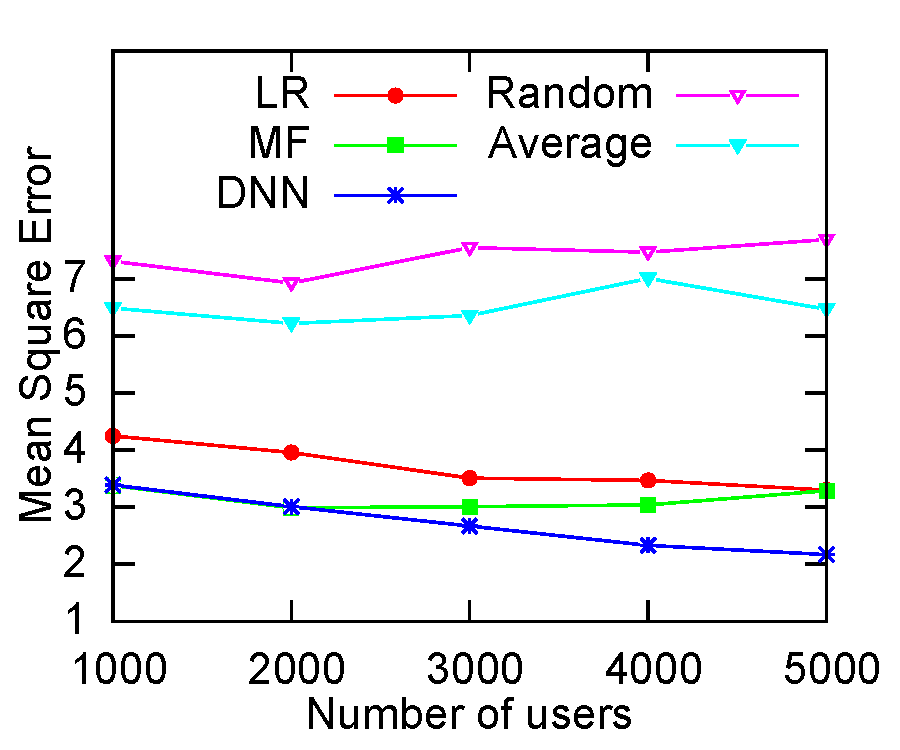
\includegraphics[scale=0.25]{E1.pdf}
        \end{subfigure}%
        ~ %add desired spacing between images, e. g. ~, \quad, \qquad, \hfill etc.
          %(or a blank line to force the subfigure onto a new line)
        \begin{subfigure}{0.25\textwidth}
                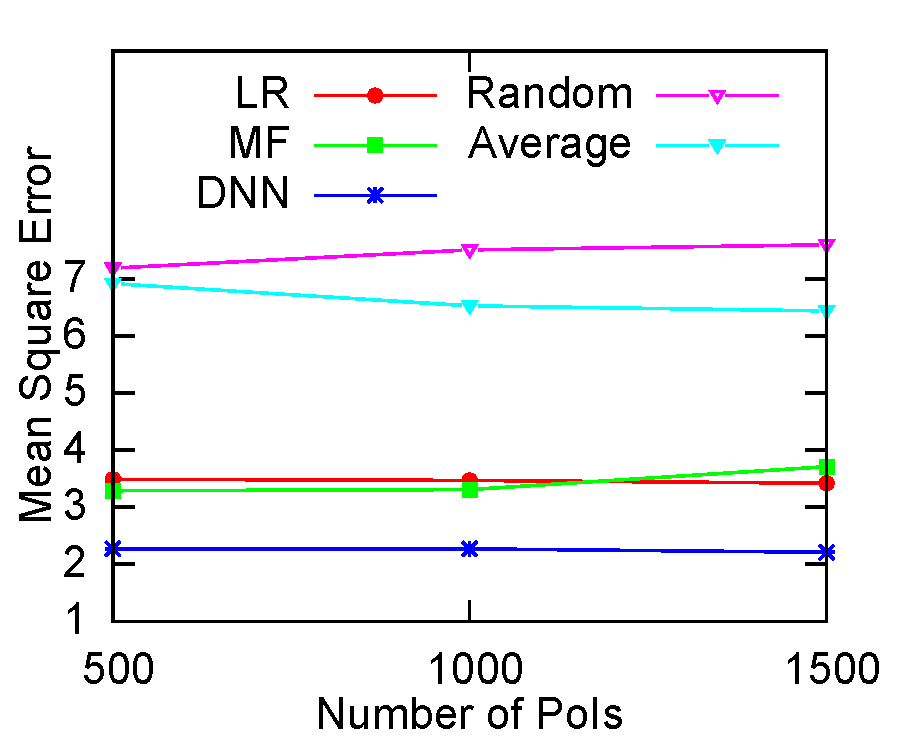
\includegraphics[scale=0.25]{E2.pdf}
        \end{subfigure}
         \caption{MSE of different prediction schemes}\label{E12}
         \vspace{-2mm}
\end{figure}

\begin{figure}[htb]%
        \centering
        \begin{subfigure}{0.25\textwidth}
               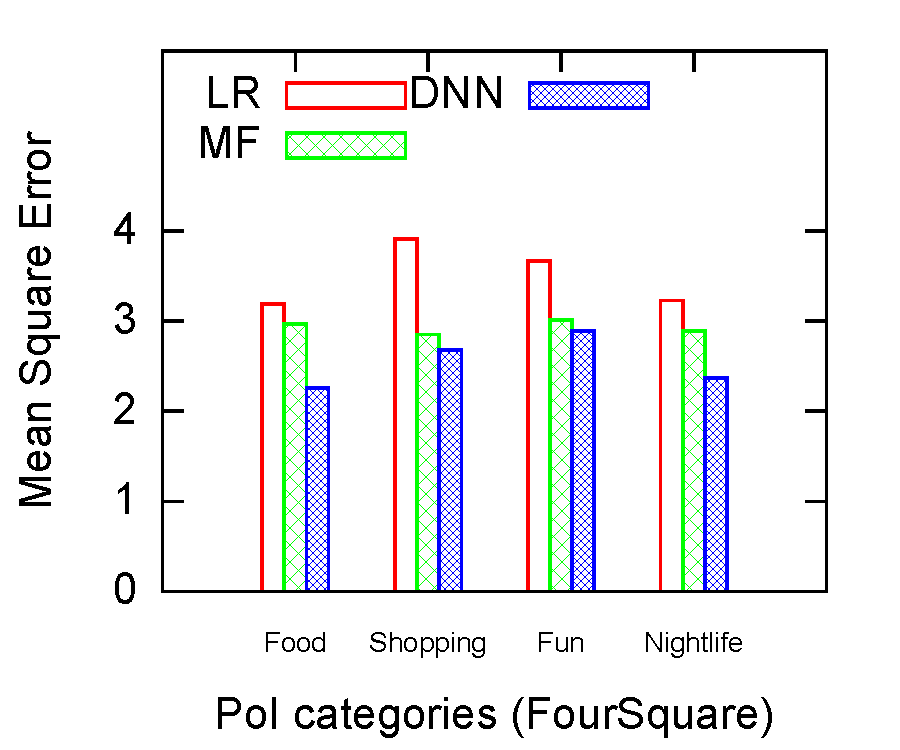
\includegraphics[scale=0.25]{E3-a.pdf}
        \end{subfigure}%
        ~ %add desired spacing between images, e. g. ~, \quad, \qquad, \hfill etc.
          %(or a blank line to force the subfigure onto a new line)
        \begin{subfigure}{0.25\textwidth}
                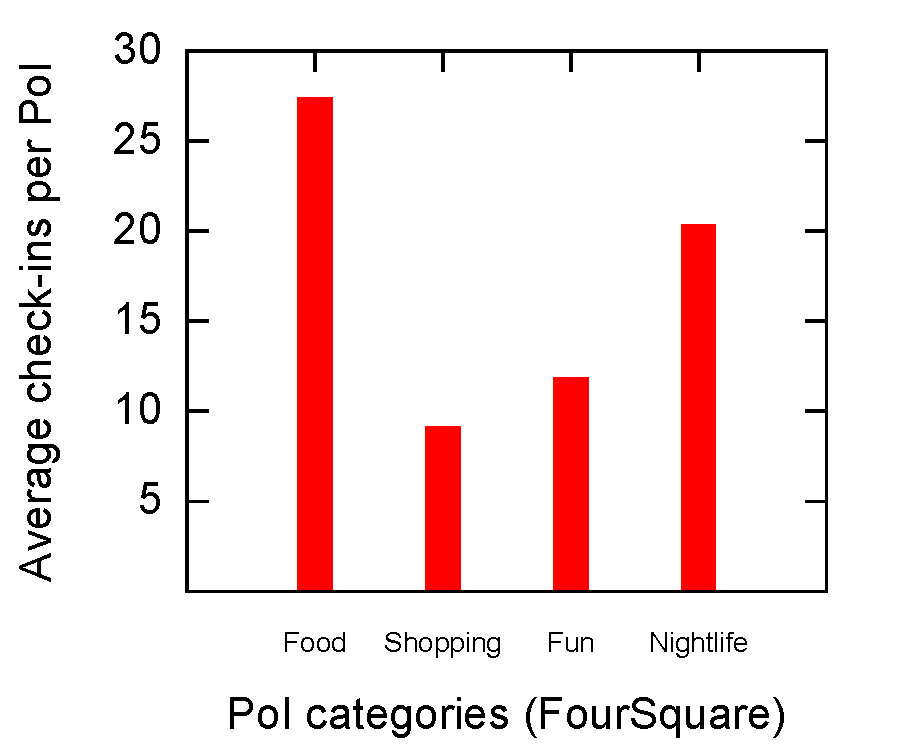
\includegraphics[scale=0.25]{E3-b.pdf}
        \end{subfigure}
         \caption{MSE of different PoI categories}\label{E3}
         \vspace{-2mm}
\end{figure}

We compare the Mean Square Error (MSE) of rating prediction results of the three schemes. We adjust the number of users and PoIs, respectively, and exam the performance trend of the compared schemes. The result is plotted in Figure~\ref{E12}. The proposed DNN prediction method demonstrate clear advantage over the other schemes for a moderate number of users. The performance of LR is also close to that of pure matrix factorization for larger number of users. The performance of DNN increases as the number of users increases. This implies a larger group of users overall have more reliable spatial-temporal features. In contrast, the performance of MF drops as the number of users/PoI increases. As the size of user-PoI rating matrix increases, it becomes more spares, making it harder for MF to generate accurate predicts. 

We also shows the MSE of the prediction result for PoIs in four different categories, namely ``Food", ``Shopping", ``Fun", and ``Nightlife". These PoI categories are provided by FourSquare. There appears to be a difference of prediction accuracy between PoI categories (Figure~\ref{E3}-a). For the proposed methods, the prediction result for ``Food" and ``Nightlife" shows a lower MSE comparing with that of ``Shopping" and ``Fun". A closer look at check-in data in different PoI category reveals that users reported less check-ins for ``Shopping" and ``Fun" PoIs comparing with that of `Food" and ``Nightlife" (Figure~\ref{E3}-b). Thus the relatively worse performance can be explained by the lack of data, which can affect the quality of extracted features.


\begin{figure}[htbp]%
        \centering
        \begin{subfigure}{0.25\textwidth}
               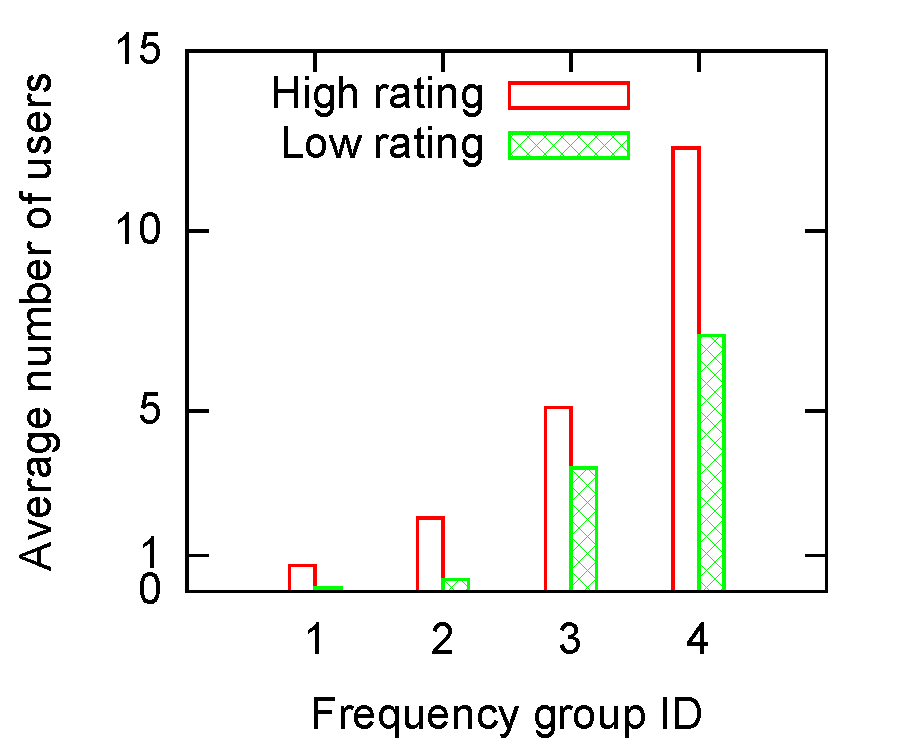
\includegraphics[scale=0.25]{E4-a.pdf}
        \end{subfigure}%
        ~ %add desired spacing between images, e. g. ~, \quad, \qquad, \hfill etc.
          %(or a blank line to force the subfigure onto a new line)
        \begin{subfigure}{0.25\textwidth}
                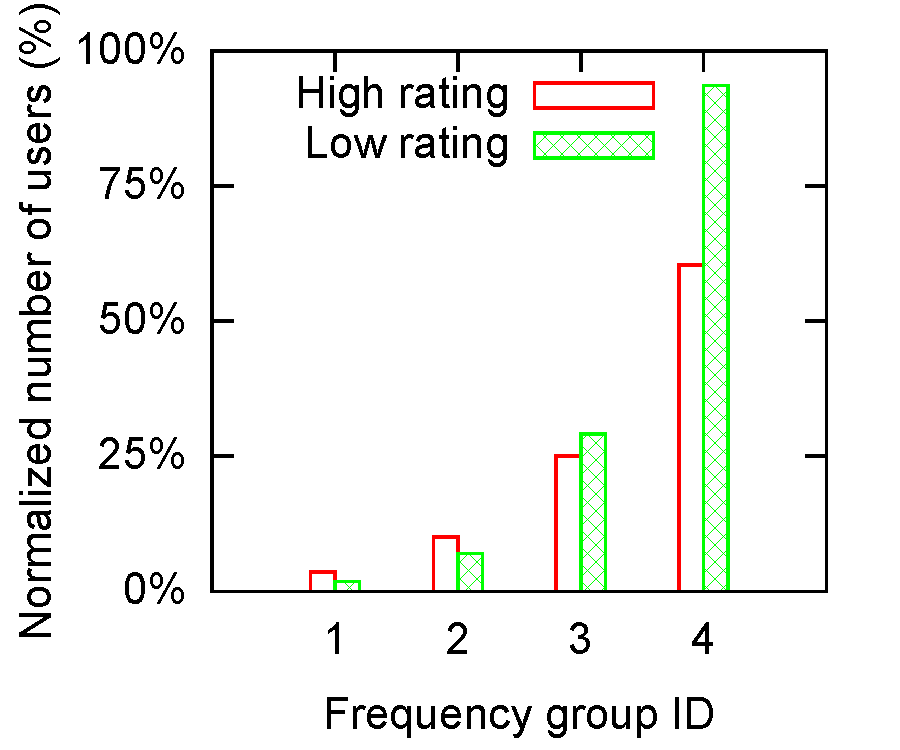
\includegraphics[scale=0.25]{E4-b.pdf}
        \end{subfigure}
         \caption{User frequency group distribution}\label{E4}
         \vspace{-2mm}
\end{figure}

Figure~\ref{E4} compares PoIs with different ratings in terms of the (normalized) average number of user in each frequency group, as showed in Table~\ref{frequencyGroups}. We define high rating PoI as a PoI with a overall score of 7.5 or higher out of 10. While a low rating PoI is one with an overall score of 2.5 or less. In general, highly rated PoIs have more visitors. Furthermore, we observe that a highly rated PoI attracts more frequent-visitors among all the visitors, comparing with PoIs with low ratings. These results support the assumptions we made in Section~\ref{sec:method}.

\vspace{-0.0cm}
\section{Conclusions}
\label{sec:conclusion}
Location-based social networks such as FourSquare, Yelp, TripAdvisor and OpenRice allow users to ``check-in'' and rate sites such as restaurants and hotels, to quantify their experience with that site. However, the vast majority of users does not use such online platforms to publish their opinion. To improve such user-site recommendation systems, we propose to exploit spatio-temporal data to estimate user-site ratings of any user. Therefore, we analysed trajectory data to find discriminative features indicating user preferences, such as their frequency of visit of a site, duration of visit, and distance from their home base. Using these features, we use existing (explicit) user-site recommendations to learn the relationship between our proposed features and the this ground-truth. Our experiments show, that our solution allows to drastically reduce the user-site-rating prediction error by exploiting spatio-temporal data. To leverage our solution to large spatio-temporal datasets, our next step is to automatically detect stay-points, rather than using pre-labelled check-in data. 


%
% The following two commands are all you need in the
% initial runs of your .tex file to

\bibliographystyle{abbrv}
\tiny{\bibliography{sigproc} } % sigproc.bib is the name of the Bibliography in this case
% You must have a proper ".bib" file
%  and remember to run:
% latex bibtex latex latex
% to resolve all references
%
% ACM needs 'a single self-contained file'!
%
%APPENDICES are optional
%\balancecolumns
%\appendix
%Appendix A
\end{document}
